% 二、研究内容及拟解决的关键问题。
% 核心比较范围按5万元申请额度收敛；具体实验参数见methods.tex。
\subsection{研究内容}
本课题以约束区域对误报与小变化检出权衡的作用为主问题。内容一确定有效样本及误差来源，内容二区分区域选择、强度和判决工作点的影响，内容三辅助检验残留错误的可识别性。检测器冻结后才开展校准和排序，并复用已有模型检查不同约束下的复核结果。三项内容的关系见图\ref{fig:mct-framework}。

\begin{center}
\begin{minipage}{\linewidth}
  \centering
  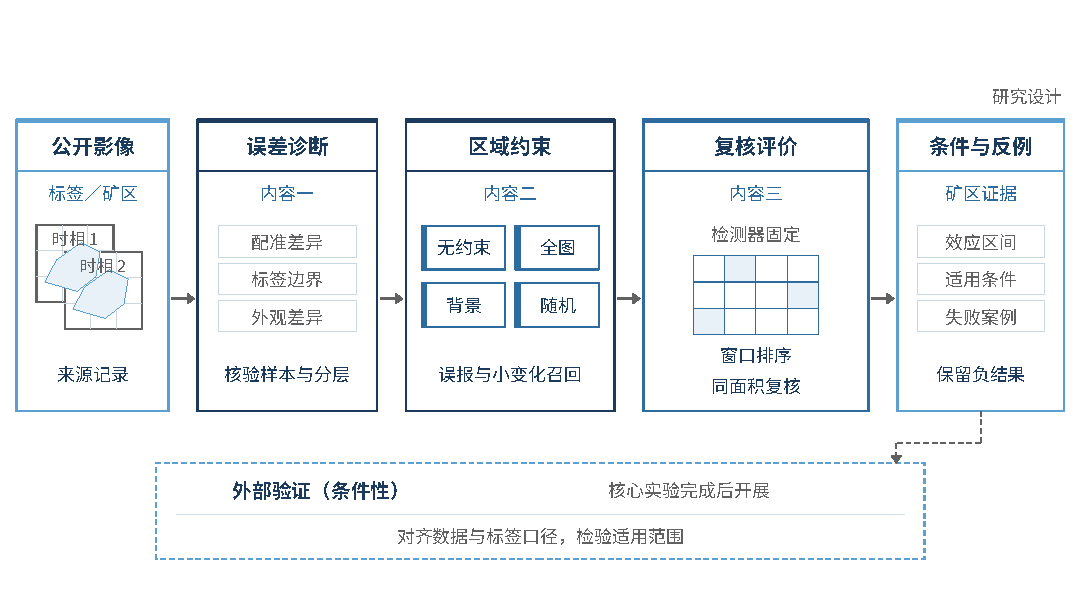
\includegraphics[width=\linewidth,trim=0 0 0 12mm,clip]{figures/vector/F02_overall_framework.pdf}
  \captionsetup{justification=justified,singlelinecheck=false}
  \captionof{figure}{总体研究框架。误差诊断向区域约束实验提供核验样本和分层规则；检测器冻结后开展复核评价，汇总适用条件与反例。外部验证为核心实验完成后的条件性扩展。}
  \label{fig:mct-framework}
\end{minipage}
\end{center}

\textbf{内容一：未见矿区变化检测的误差诊断。}
以MineNetCD为主数据，核对矿区、原始影像与切片来源，沿用官方矿区分组建立训练、校准、验证和测试协议。复现ResNet-18孪生基线后，按矿区分析误报与漏检，抽查高置信度误检、漏检和随机正常样本，区分配准差异、标签边界、背景外观差异与真实细小变化。据此判断错误是否与一致性约束相关，确定机制实验的分层标准和比较对象。

\textbf{内容二：跨时相一致性约束的作用区域与负迁移条件。}
同一骨干的无约束、全图、背景和随机区域四组承担主比较，检验误报及细小变化召回的权衡。固定模型与面积后改变掩码中的变化比例，分析特征距离与监督梯度；结合强度匹配、平滑及阈值敏感性对照解释结果。完整DonaNet与其区域替换用于检验适用性。最多6次额外训练优先保障强度匹配；FCCDN、CDDGNet等扩展须在主问题所需对照完成且有余量时开展，不以简化消融代表原方法。

\textbf{内容三：固定复核面积下的可靠性评价。}
固定检测器后，在独立矿区校准概率，结合概率熵与固定多视图推理分歧对全图有效窗口排序，比较同一面积预算下的剩余误报与漏检，检查高置信度未变化预测中的错误。理想纠错模拟用于估计复核效果上限；合作者落实后开展小规模真实复核，分别记录面积、窗口数和工时。EuroMineNet作为条件性扩展，验证其内部未见矿区的适用性。

\subsection{研究目标}
总体目标是在公开矿山数据上解释一致性约束对变化判别的条件性作用，并检验预测可靠性信息能否帮助识别未见矿区的错误。

一是建立可复现的矿区级误差诊断与对照协议，明确数据条件。二是检验背景限定约束相对同骨干全图约束能否改善误报并保持细小变化召回非劣，识别成立或失效的范围。三是量化错误排序相对随机和单指标基线的复核收益与代价，报告全图剩余错误及变化覆盖。以效应量、区间和对照结果衡量目标完成情况，不承诺缺少前测依据的精度涨幅。

\subsection{拟解决的关键科学问题}
\textbf{问题一：约束区域如何影响变化敏感性？}
未变化地物的两期特征差异可能包含观测干扰，真实变化的特征差异则承载判别信息。同一一致性目标在两类区域中可能产生不同作用。本项目通过固定面积的约束污染实验和自然矿区分层，分析变化比例、变化尺度及外观差异如何影响这种作用，并检验总体正则强度能否单独解释结果。

\textbf{问题二：概率与推理稳定性能够识别哪些预测错误？}
即使校准概率接近经验正确率，仍可能遗漏高置信度漏检。本课题比较概率熵和多视图分歧发现的错误及其互补条件，检验低复核预算下组合排序能否同时发现误报与漏检，避免仅减少易发现的误报而遗漏真实变化。

\textbf{上述问题的共同边界：在何种矿区和观测条件下能够重现？}
以矿区为独立评估单位，分析不同外观差异和变化尺度下的效应及反例。跨数据集比较前先对齐输入与标签口径，再判断结果能否重现，并区分观测系统差异与算法泛化机制的影响。
